\def\pcscwp{
Center for Wave Phenomena \\ 
Colorado School of Mines \\ 
psava@mines.edu
}

\def\pcscover{
\author[]{Paul Sava}
\institute{\pcscwp}
\date{}
\logo{WSI}
\large
}

\def\WSI{\textbf{WSI}~}

% ------------------------------------------------------------
% colors
\def\red#1{\textcolor{red}{#1}}
\def\green#1{\textcolor{green}{#1}}
\def\blue#1{\textcolor{blue}{#1}}
\def\yellow#1{\textcolor{yellow}{#1}}
\def\magenta#1{\textcolor{magenta}{#1}}

\def\black#1{\textcolor{black}{#1}}
\def\white#1{\textcolor{white}{#1}}
\def\gray#1{\textcolor{gray}{#1}}

\definecolor{DarkGreen}{rgb}{0,0.5,0}
\definecolor{DarkBlue}{rgb}{0,0,0.5}
\definecolor{DarkRed}{rgb}{0.5,0,0}
\definecolor{DarkYellow}{rgb}{0.5,0,0}
\definecolor{LightRed}{rgb}{1.000,0.752,0.796}
\definecolor{LightGreen}{rgb}{0.792,1.000,0.439}
\definecolor{LightBlue}{rgb}{0.690,0.886,1.000}
\definecolor{LightYellow}{rgb}{1.000,0.925,0.545}
\definecolor{DarkGray}{rgb}{0.45,0.45,0.45}
\definecolor{LightGray}{rgb}{0.90,0.90,0.90}

\def\darkgreen#1{\textcolor{DarkGreen}{#1}}
\def\darkblue#1 {\textcolor{DarkBlue}{#1}}
\def\darkred#1  {\textcolor{DarkRed}{#1}}
\def\lightred#1 {\textcolor{LightRed}{#1}}

\def\lightgray#1{\textcolor{LightGray}{#1}}
\def\darkgrey#1 {\textcolor{DarkGray}{#1}}

% ------------------------------------------------------------
% madagascar
\def\mg{\darkgreen{\sc madagascar~}}
\def\latex{\darkgreen{\sc \LaTeX}}
\def\mex#1{ \normalsize \red{ \texttt{#1} } \large }
\def\mvbt#1{\small{\blue{\begin{semiverbatim}#1\end{semiverbatim}}}}

% ------------------------------------------------------------
% equations
\def\bea{\begin{eqnarray}}
\def\eea{  \end{eqnarray}}

\def\beq{\begin{equation}}
\def\eeq{  \end{equation}}

%\def\req#1{(\ref{#1})}

\def\lp{\left (}
\def\rp{\right)}

\def\lb{\left [}
\def\rb{\right]}

\def\pbox#1{ \fbox {$ \displaystyle #1 $}}

\def\non{\nonumber \\ \nonumber}

% ------------------------------------------------------------
% REFERENCE (equations and figures)
\def\rEq#1{Equation~\ref{eqn:#1}}
\def\req#1{equation~\ref{eqn:#1}}
\def\rEqs#1{Equations~\ref{eqn:#1}}
\def\reqs#1{equations~\ref{eqn:#1}}
\def\ren#1{\ref{eqn:#1}}

\def\rFg#1{Figure~\ref{fig:#1}}
\def\rfg#1{Figure~\ref{fig:#1}}
\def\rFgs#1{Figures~\ref{fig:#1}}
\def\rfgs#1{Figures~\ref{fig:#1}}
\def\rfn#1{\ref{fig:#1}}

% ------------------------------------------------------------
% field operators

% trace
\def\tr{\texttt{tr}\;}

% divergence
\def\DIV#1{\nabla \cdot {#1}}

% curl
\def\CURL#1{\nabla \times {#1}}

% gradient
\def\GRAD#1{\nabla {#1}}

% Laplacian
\def\LAPL#1{\nabla^2 {#1}}

\def\dellin{
\lb
\begin{matrix}
\done{}{x} \; \done{}{y} \; \done{}{z}
\end{matrix}
\rb
}

\def\delcol{
\lb
\begin{matrix}
\done{}{x} \non
\done{}{y} \non
\done{}{z}
\end{matrix}
\rb
}

\def\aveclin{
\lb
\begin{matrix}
a_x \; a_y \; a_z
\end{matrix}
\rb
}


% ------------------------------------------------------------

% elastic tensor
\def\CC{{\bf C}}

% identity tensor
\def\I{\;{\bf I}}

% particle displacement vector
\def\uu{{\bf u}}

% particle velocity vector
\def\vv{{\bf v}}

% particle acceleration vector
\def\aa{{\bf a}}

% force vector
\def\ff{{\bf f}}

% wavenumber vector
\def\kk{{\bf k}}

% ray parameter vector
\def\pp{{\bf p}}

% distance vector
\def\xx{{\bf x}}
\def\kkx{{\kk_\xx}}
\def\ppx{{\pp_\xx}}

\def\yy{{\bf y}}

% normal vector
\def\nn{{\bf n}}
\def\ns{\nn_s}
\def\nr{\nn_r}

% source vector
\def\ss{{\bf s}}
\def\kks{{\kk_\ss}}
\def\pps{{\pp_\ss}}

% receiver vector
\def\rr{{\bf r}}
\def\kkr{{\kk_\rr}}
\def\ppr{{\pp_\rr}}

% midpoint vector
\def\mm{{\bf m}}
\def\kkm{{\kk_\mm}}
\def\ppm{{\pp_\mm}}

% offset vector
\def\ho{{\bf h}}
\def\kkh{{\kk_\ho}}
\def\pph{{\pp_\ho}}

% space-lag vector
\def\hh{ {\boldsymbol{\lambda}} }
\def\kkl{{\kk_\hh}}
\def\ppl{{\pp_\hh}}

% CIP vector
\def\cc{ {\bf c}}

% time-lag scalar
\def\tt{\tau}
\def\tts{\tt_s}
\def\ttr{\tt_r}

% frequency
\def\ww{\omega}

%
\def\dd{{\bf d}}

\def\bb{{\bf b}}
\def\qq{{\bf q}}

\def\ii{{\bf i}} % unit vector
\def\jj{{\bf j}} % unit vector

\def\lo{{\bf l}}

% ------------------------------------------------------------

\def\Fop#1{\mathcal{F}     \lb #1 \rb}
\def\Fin#1{\mathcal{F}^{-1}\lb #1 \rb}

% ------------------------------------------------------------
% partial derivatives

\def\dtwo#1#2{\frac{\partial^2 #1}{\partial #2^2}}
\def\done#1#2{\frac{\partial   #1}{\partial #2  }}
\def\dthr#1#2{\frac{\partial^3 #1}{\partial #2^3}}
\def\mtwo#1#2#3{ \frac{\partial^2#1}{\partial #2 \partial#3} }

\def\larrow#1{\stackrel{#1}{\longleftarrow}}
\def\rarrow#1{\stackrel{#1}{\longrightarrow}}

% ------------------------------------------------------------
% elasticity 

\def\stress{\underline{\textbf{t}}}
\def\strain{\underline{\textbf{e}}}
\def\stiffness{\underline{\underline{\textbf{c}}}}
\def\compliance{\underline{\underline{\textbf{s}}}}

\def\GEOMlaw{
\strain = \frac{1}{2} 
\lb \GRAD{\uu} + \lp \GRAD{\uu} \rp^T \rb
}

\def\HOOKElaw{
\stress = \lambda \; tr \lp \strain \rp {\bf I} + 2 \mu \strain 
}

\def\CONSTITUTIVElaw{
\stress = \stiffness \;\strain 
}


\def\NEWTONlaw{
\rho \ddot{\uu} = \DIV{\stress}
}

\def\NAVIEReq{
\rho \ddot\uu =
\lp \lambda + 2\mu \rp \GRAD{\lp \DIV{\uu} \rp}
             - \mu     \CURL{   \CURL{\uu}}
}

% ------------------------------------------------------------

% potentials
\def\VP{\boldsymbol{\psi}}
\def\SP{\theta}

% stress tensor
\def\ssten{{\bf \sigma}}

\def\ssmat{
\lp \matrix {
 \sigma_{11} &  \sigma_{12}   &  \sigma_{13} \cr
 \sigma_{12} &  \sigma_{22}   &  \sigma_{23} \cr
 \sigma_{13} &  \sigma_{23}   &  \sigma_{33} \cr
} \rp
}

% strain tensor
\def\eeten{{\bf \epsilon}}

\def\eemat{
\lp \matrix {
 \epsilon_{11} &  \epsilon_{12}   &  \epsilon_{13} \cr
 \epsilon_{12} &  \epsilon_{22}   &  \epsilon_{23} \cr
 \epsilon_{13} &  \epsilon_{23}   &  \epsilon_{33} \cr
} \rp
}


% plane wave kernel
\def\pwker{A e^{i k \lp \nn \cdot \xx - v t \rp}}


% ------------------------------------------------------------
% details for expert audience (math, cartoons)
\def\expert{
\colorbox{red}{\textbf{\LARGE \white{!}}}
}

% ------------------------------------------------------------
% image, data, wavefields

\def\RR{R}

\def\UU{W}
\def\US{{\UU_s}}
\def\UR{{\UU_r}}

\def\DD{D}
\def\DS{{\DD_s}}
\def\DR{{\DD_r}}

\def\UUw{\UU}
\def\USw{{\UU_s}}
\def\URw{{\UU_r}}

\def\DDw{\DD}
\def\DSw{{\DD_s}}
\def\DRw{{\DD_r}}

% perturbations

\def\ds{\Delta s}
\def\dl{\Delta l}
\def\di{\Delta \RR}
\def\du{\Delta \UU}

\def\dRR{\Delta \RR}
\def\dUU{\Delta \UU}
\def\dUS{\Delta \US}
\def\dUR{\Delta \UR}

\def\dtt{\Delta \tt}
\def\dhh{\Delta \hh}

% ------------------------------------------------------------
% Green's functions

\def\GG{G}

\def\GS{{\GG_s}}
\def\GR{{\GG_r}}

% ------------------------------------------------------------
% elastic data, wavefields

\def\eRR{\textbf{\RR}}

\def\eDS{{\textbf{\DD}_s}}
\def\eDR{{\textbf{\DD}_r}}
\def\eDD{{\textbf{\DD}}}

\def\eUS{{\textbf{\UU}_s}}
\def\eUR{{\textbf{\UU}_r}}
\def\eUU{{\textbf{\UU}}}

% ------------------------------------------------------------
% sliding bar
\def\tline#1{
\put(95,-3){\small \blue{time}}
\put(-4,-1){\small \blue{0}}
\thicklines
\put( 0,0){\color{blue} \vector(1,0){100}}
\put(#1,0){\color{red}  \circle*{2}}
}

% ------------------------------------------------------------
% arrow on figure
\def\myarrow#1#2#3{
\thicklines
\put(#1,#2){\color{green} \vector(-1,-1){5}}
\put(#1,#2){\color{green} \textbf{#3}}
}

\def\bkarrow#1#2#3{
\thicklines
\put(#1,#2){\color{black} \vector(-1,-1){5}}
\put(#1,#2){\color{black} \textbf{#3}}
}

\def\anarrow#1#2#3#4{
\thicklines
\put(#1,#2){\color{#4} \vector(-1,-1){5}}
\put(#1,#2){\color{#4} \textbf{#3}}
}

\def\myvec#1#2#3#4{
\thicklines
\put(#1,#2){\color{green} \rotatebox{#4}{\vector(4,0){20}}}
\put(#1,#2){\color{green} \textbf{#3}}
}

% ------------------------------------------------------------
% circle on figure
\def\mycircle#1#2#3{
\thicklines
\put(#1,#2){\color{green} \circle{#3}}
}

% ------------------------------------------------------------
% note on figure
\def\mynote#1#2#3{
\put(#1,#2){\color{green} \textbf{#3}}
}

\def\biglabel#1#2#3{
\put(#1,#2){\Large \textbf{#3}}
}

\def\wlabel#1#2#3{ \white{ \biglabel{#1}{#2}{#3} }}
\def\klabel#1#2#3{ \black{ \biglabel{#1}{#2}{#3} }}
\def\rlabel#1#2#3{ \red{   \biglabel{#1}{#2}{#3} }}
\def\glabel#1#2#3{ \green{ \biglabel{#1}{#2}{#3} }}
\def\blabel#1#2#3{ \blue { \biglabel{#1}{#2}{#3} }}
\def\ylabel#1#2#3{ \yellow{\biglabel{#1}{#2}{#3} }}

% ------------------------------------------------------------
% centering
\def\cen#1{ \begin{center} \textbf{#1} \end{center}}
\def\cit#1{ \begin{center} \textit{#1} \end{center}}
\def\ctt#1{ \begin{center} \texttt{#1} \end{center}}

% emphasis (bold+alert)
\def\bld#1{ \textbf{\alert{#1}}}

% huge fonts
\def\big#1{\begin{center} {\LARGE \textbf{#1}} \end{center}}
\def\hug#1{\begin{center} {\Huge  \textbf{#1}} \end{center}}

% ------------------------------------------------------------
% separator
\def\sep{ \vfill \hrule \vfill}
\def\itab{ \hspace{0.5in}}
\def\nsp{\\ \vspace{0.1in}}

% ------------------------------------------------------------
% integrals

\def\tint#1{\!\!\!\int\!\! #1 dt}
\def\xint#1{\!\!\!\int\!\! #1 d\xx}
\def\wint#1{\!\!\!\int\!\! #1 d\ww}
\def\aint#1{\!\!\!\alert{\int}\!\! #1 d\alert{\xx}}

\def\esum#1{\sum\limits_{#1}}
\def\eint#1{\int\limits_{#1}}

% ------------------------------------------------------------
\def\CONJ#1{\overline{#1}}
\def\MOD#1{\left| {#1} \right|}

% ------------------------------------------------------------
% imaging components

\def\IC{\colorbox{yellow}{\textbf{I.C.}}\;}
\def\WR{\colorbox{yellow}{\textbf{W.R.}}\;}
\def\WE{\colorbox{yellow}{\textbf{W.E.}}\;}
\def\SO{\colorbox{yellow}{\textbf{SOURCE}}\;}
\def\WS{\colorbox{yellow}{\textbf{W.S.}}\;}

% ------------------------------------------------------------
% summary/take home message
\def\thm{take home message}

% ------------------------------------------------------------
\def\dx{\Delta x}
\def\dy{\Delta y}
\def\dz{\Delta z}
\def\dt{\Delta t}

\def\dhx{\Delta h_x}
\def\dhy{\Delta h_y}

\def\kz{{k_z}}
\def\kx{{k_x}}
\def\ky{{k_y}}

\def\kmx{k_{m_x}}
\def\kmy{k_{m_y}}
\def\khx{k_{h_x}}
\def\khy{k_{h_y}}

\def\why{ \alert{\widehat{{\khy}}}}
\def\whx{ \alert{\widehat{{\khx}}}}

\def\lx{{\lambda_x}}
\def\ly{{\lambda_y}}
\def\lz{{\lambda_z}}

\def\klx{k_{\lambda_x}}
\def\kly{k_{\lambda_y}}
\def\klz{k_{\lambda_z}}

\def\mx{{m_x}}
\def\my{{m_y}}
\def\mz{{m_z}}
\def\hx{{h_x}}
\def\hy{{h_y}}
\def\hz{{h_z}}

\def\sx{{s_x}}
\def\sy{{s_y}}
\def\rx{{r_x}}
\def\ry{{r_y}}

% ray parameter (absolute value)
\def\modp#1{\left| \pp_{#1} \right|}

% wavenumber
\def\modk#1{\left| \kk_{#1} \right|}

% ------------------------------------------------------------
\def\kzwk{ {\kz^{\kk}}}
\def\kzwx{ {\kz^{\xx}}}
 
\def\PSk#1{e^{\red{#1 i \kzwk \dz}}}
\def\PSx#1{e^{\red{#1 i \kzwx \dz}}}
\def\PS#1{ e^{\red{#1 i k_z   \dz}}}

\def\TT{t}
\def\TS{t_s}
\def\TR{t_r}

\def\oft{\lp t \rp}
\def\ofw{\lp \ww \rp}

\def\ofx{\lp \xx \rp}
\def\ofh{\lp \hh \rp}
\def\ofk{\lp \kk \rp}
\def\ofs{\lp \ss \rp}
\def\ofr{\lp \rr \rp}
\def\ofz{\lp   z \rp}

\def\ofxt{\lp \xx, t  \rp}
\def\ofst{\lp \ss, t  \rp}
\def\ofrt{\lp \rr, t  \rp}

\def\ofxw{\lp \xx, \ww  \rp}
\def\ofsw{\lp \ss, \ww  \rp}
\def\ofrw{\lp \rr, \ww  \rp}

\def\ofxm{\lp \xx,\hh \rp}

\def\ofxmp{\lp \xx+\hh \rp}
\def\ofxmm{\lp \xx-\hh \rp}

\def\ofmm{\lp \mm      \rp}
\def\ofmz{\lp \mm, z   \rp}
\def\ofmw{\lp \mm, \ww \rp}
\def\ofkm{\lp \kkm     \rp}

% ------------------------------------------------------------
% source/receiver data and wavefields

\def\dst{$\DS\ofst$}
\def\drt{$\DR\ofrt$}
\def\ust{$\US\ofxt$}
\def\urt{$\UR\ofxt$}

\def\dsw{$\DS\ofsw$}
\def\drw{$\DR\ofrw$}
\def\usw{$\US\ofxw$}
\def\urw{$\UR\ofxw$}

% ------------------------------------------------------------
\def\Nx{N_x}
\def\Ny{N_y}
\def\Nz{N_z}
\def\Nt{N_t}
\def\Nw{N_{\ww}}
\def\Nm{N_{\mm}}

\def\Nlx{N_{\lambda_x}}
\def\Nly{N_{\lambda_y}}
\def\Nlz{N_{\lambda_z}}
\def\Nlt{N_{\tau}}

\def\wmin{\ww_{min}}
\def\wmax{\ww_{max}}
\def\zmin{z_{min}}
\def\zmax{z_{max}}
\def\tmin{t_{min}}
\def\tmax{t_{max}}
\def\lmin{\hh_{min}}
\def\lmax{\hh_{max}}
\def\xmin{\xx_{min}}
\def\xmax{\xx_{max}}

% ------------------------------------------------------------
% course qualifiers

\def\fun{\hfill \alert{concepts}}
\def\pra{\hfill \alert{applications}}
\def\fro{\hfill \alert{frontiers}}


% ------------------------------------------------------------
% wavefield extrapolation
\def\ws{ {\ww s} }

\def\kows{\lp \frac{\kx}{\ws} \rp}

\def\kmws{\lp \frac{\modk{\mm}}{\ws} \rp}
\def\kzws{\lp \frac{\kz}       {\ws} \rp}

\def\S{\lb\frac{\modk{\mm}}{\ws  }\rb}
\def\C{\lb\frac{\modk{\mm}}{\ws_0}\rb}
\def\K{\lb\frac{\modk{\mm}}{\ww  }\rb}

\def\Cs{\lb\frac{\modk{\mm}^2}{\lp \ws_0 \rp^2}\rb}

\def\SSR#1{  \sqrt{ \lp \ww {#1} \rp^2 - \modk{\mm}^2} }

\def\SQRsum#1{\sum\limits_{n=1}^{\infty} \lp -1 \rp^n
		\displaystyle{\frac{1}{2} \choose n} #1}

\def\TSE#1#2#3#4{\sum\limits_{#4=#3}^{\infty} \lp -1 \rp^#4
		\displaystyle{#2 \choose #4} {#1}^#4}

\def\onefrac#1#2{\frac{#2^2}{a_#1+b_#1 #2^2}}
\def\SQRfrac#1{
	\sum\limits_{n=1}^{\infty}
	\onefrac{n}{#1} }

\def\dkzds { \left. \frac{d {\kz}}  {d s} \right|_{s_b} }
\def\SSX#1#2{\sqrt{ 1 - \lb \frac{\MOD{#2}}{#1} \rb^2} }
\def\SST#1#2{1 + \sum_{j=1}^N c_j \lb \frac{\MOD{#2}}{#1} \rb^{2j} }

% ------------------------------------------------------------
% acknowledgment
\def\ackcwp{\cen{the sponsors of the\\Center for Wave Phenomena\\at\\Colorado School of Mines}}

% ------------------------------------------------------------
% citation in slides
\def\talkcite#1{{\small \sc #1}}

% ------------------------------------------------------------
\def\ise{GPGN302: Introduction to EM and Seismic Exploration}
\def\inv{GPGN409: Inversion}

% ------------------------------------------------------------
\def\model{m}
\def\data {d}

\def\Lop{ {\mathbf{L}}}
\def\Sop{ {\mathbf{S}}}
\def\Eop{ {\mathbf{E}}}
\def\Iop{ {\mathbf{I}}}
\def\Aop{ {\mathbf{A}}}
\def\Pop{ {\mathbf{P}}}
\def\Fop{ {\mathbf{F}}}
\def\Kop{ {\mathbf{K}}}


% ------------------------------------------------------------
\def\mybox#1{
  \begin{center}
    \fcolorbox{black}{yellow}
    {\begin{minipage}{0.8\columnwidth} {#1} \end{minipage}}
  \end{center}
}

\def\hibox#1{
  \begin{center}
    \fcolorbox{black}{LightGreen}
    {\begin{minipage}{0.8\columnwidth} {#1} \end{minipage}}
  \end{center}
}

% ------------------------------------------------------------
% Nota Bene
\def\nbnote#1{
  \vfill
  \begin{center}
    \colorbox{LightGray}
    {\begin{minipage}{\columnwidth} {\textbf{\black{\large N.B.}} #1} \end{minipage}}
  \end{center}
}

\def\notabene#1{
  \begin{leftbar}
    {\sc Nota Bene:~} #1
  \end{leftbar}
}

\def\sidebar#1{
  \begin{leftbar}
    {#1}
  \end{leftbar}
}


\def\highlight#1{
  \begin{center}
    \colorbox{LightRed}
    {\begin{minipage}{0.95\columnwidth} {#1} \end{minipage}}
  \end{center}
}

% ------------------------------------------------------------
\def\pcsshaded#1{
  \definecolor{shadecolor}{rgb}{0.8,0.8,0.8}
  \begin{shaded} {#1} \end{shaded}
  \definecolor{shadecolor}{rgb}{1.0,1.0,1.0}
}

\def\blueshade#1{
  \definecolor{shadecolor}{rgb}{0.690,0.886,1.000}
    \begin{shaded}
      {#1}
    \end{shaded}
  \definecolor{shadecolor}{rgb}{1.0,1.0,1.0}
}

\def\grayshade#1{
  \definecolor{shadecolor}{rgb}{0.8,0.8,0.8}
  \begin{shaded}
    {#1}
  \end{shaded}
  \definecolor{shadecolor}{rgb}{1.0,1.0,1.0}
}

\def\yellowshade#1{
  \definecolor{shadecolor}{rgb}{1.0,1.0,0.0}
  \begin{shaded}
    {#1}
  \end{shaded}
  \definecolor{shadecolor}{rgb}{1.0,1.0,1.0}
}


% ------------------------------------------------------------
\def\postit#1{
  \begin{center}
    \colorbox{yellow}
    {\begin{minipage}{0.80\columnwidth} {#1} \end{minipage}} 
  \end{center}
}

% ------------------------------------------------------------
\def\graybox#1{
  \begin{center}
    \colorbox{LightGray}
    {\begin{minipage}{1.00\columnwidth} {#1} \end{minipage}}
  \end{center}
}

\def\whitebox#1{
  \begin{center}
    \colorbox{white}
    {\begin{minipage}{1.00\columnwidth} {#1} \end{minipage}}
  \end{center}
}

\def\yellowbox#1{
  \begin{center}
    \colorbox{LightYellow}
    {\begin{minipage}{1.00\columnwidth} {#1} \end{minipage}}
  \end{center}
}

\def\greenbox#1{
  \begin{center}
    \colorbox{LightGreen}
    {\begin{minipage}{1.00\columnwidth} {#1} \end{minipage}}
  \end{center}
}

\def\bluebox#1{
  \begin{center}
    \colorbox{LightBlue}
    {\begin{minipage}{1.00\columnwidth} {#1} \end{minipage}}
  \end{center}
}

\def\redbox#1{
  \begin{center}
    \colorbox{LightRed}
    {\begin{minipage}{1.00\columnwidth} {#1} \end{minipage}}
  \end{center}
}

\def\hyellow#1{ \colorbox{yellow} #1 }
\def\hgreen #1{ \colorbox{green}  #1 }

% ------------------------------------------------------------
% boxes for vectors and matrices

\def\pcsbox#1#2#3#4{
  % #1 = hmax
  % #2 = height
  % #3 = width
  % #4 = text
  \begin{picture}(#3,#1)
    \linethickness{0.5mm}
    % 
    \multiput(0,#1)(#3, 0){2}{\line(0,-1){#2}}
    \multiput(0,#1)(0,-#2){2}{\line(+1,0){#3}}
    % 
    \put(1,-10){#4}
  \end{picture}
}

% annotate block equations
\def\pcssym#1#2{
  \begin{picture}(3,#1)
    \put(1,-10){#2}
  \end{picture}
}

% block equation sign
\def\pcsops#1#2#3#4{
  \begin{picture}(#3,#1)
    \put(0,#2){#4}
  \end{picture}
}

% ------------------------------------------------------------
% two color boxes
\def\sidebyside#1#2{
  \begin{center}
    \colorbox{LightBlue}{
      \begin{minipage}{1.0\columnwidth} {#1} \end{minipage}
    }
    \colorbox{LightYellow}{
      \begin{minipage}{1.0\columnwidth} {#2} \end{minipage}
    }
  \end{center}
}

% upward pointing arrow
\def\uparrow#1#2#3{
  \thicklines
  \put(#1,#2){\color{green} \vector(0,+1){5}}
  \put(#1,#2){\color{green} \textbf{#3}}
}

% acknowledge figure source
\def\ackfig#1#2#3{\blabel{#1}{#2}{\normalsize \sc #3}}


\pgfdeclareimage[height=1.0in]{logo}{Fig/kaust}

\title[]{Writing a paper}
\subtitle{using Madagascar}
\author{Tariq Alkhalifah} 
\institute{
Seismic Analysis Group (SWAG) \\
KAUST \\
swag.kaust.edu.sa
}
\date{}
%\logo{Fig/swag_logo}
% ------------------------------------------------------------
\mode<beamer> { \cwpcover }

\def\beq{\begin{equation}}
\def\eeq{\end{equation}}
\def\beqa{\begin{eqnarray}}
\def\eeqa{\end{eqnarray}}

% ------------------------------------------------------------
\inputdir{XFig}
% ------------------------------------------------------------

\begin{frame} 
\frametitle{From the net}

\big{
Q: What is the difference between a Ph.D. in mathematics and a large pizza?
A: A large pizza can feed a family of four... 
}

\end{frame}
\cwpnote{}

% ------------------------------------------------------------
\begin{frame} 

\frametitle{Top 10 reasons why Professor Sergey called this package Madagascar}

\begin{itemize}
\item 10. He was in Madagascar, so he said what the heck.
\item 9. The only country he did not travel to.
\item 8. All the vowels are ``a'', which made it easier to spell.
\item 7. It is the only country he could spell.
\item 6. If you break it down ``Mad'' ``a'' ``gas'' ``car'', related
  to the Oil industry.
\item .........
\end{itemize}

\end{frame}
\cwpnote{}

% ------------------------------------------------------------
\begin{frame} 

\frametitle{Writing papers, what will we learn?}

\big{
\begin{itemize}
\item Use Madagascar to write papers.
\item The template concept.
\item The scons role.
\item Reproducible.
\item The book (file system).
\end{itemize}
}

\end{frame}
\cwpnote{}

% ------------------------------------------------------------
\begin{frame} 

\frametitle{Challenges}

\big{
The seemingly complex makeup:
\begin{itemize}
\item LaTeX, python (scons????), and C.
\item The file system (where is everything?).
\item incomplete and not-up-to-date documentation.
\item Any info on the libraries? (C and Python)?
\end{itemize}
}

\end{frame}
\cwpnote{}

% ------------------------------------------------------------
\begin{frame} 

\frametitle{A general objective}

\big{
\begin{itemize}
\item Getting from Madagascar what you need: even if we have to get dirty.
\item Example subject: Traveltime sensitivity kernels 
\end{itemize}
}

\end{frame}
\cwpnote{}

\begin{frame}
  \frametitle{The Big Scheme of Things}
  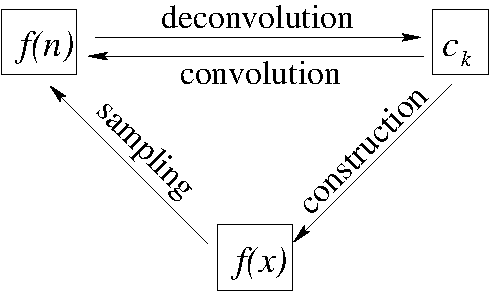
\includegraphics[height=0.8\textheight]{XFig/Fig/scheme} \\
Courtesy of Fomel (2006)
\end{frame}

\begin{frame}
  \frametitle{The Big Scheme of Things II}
  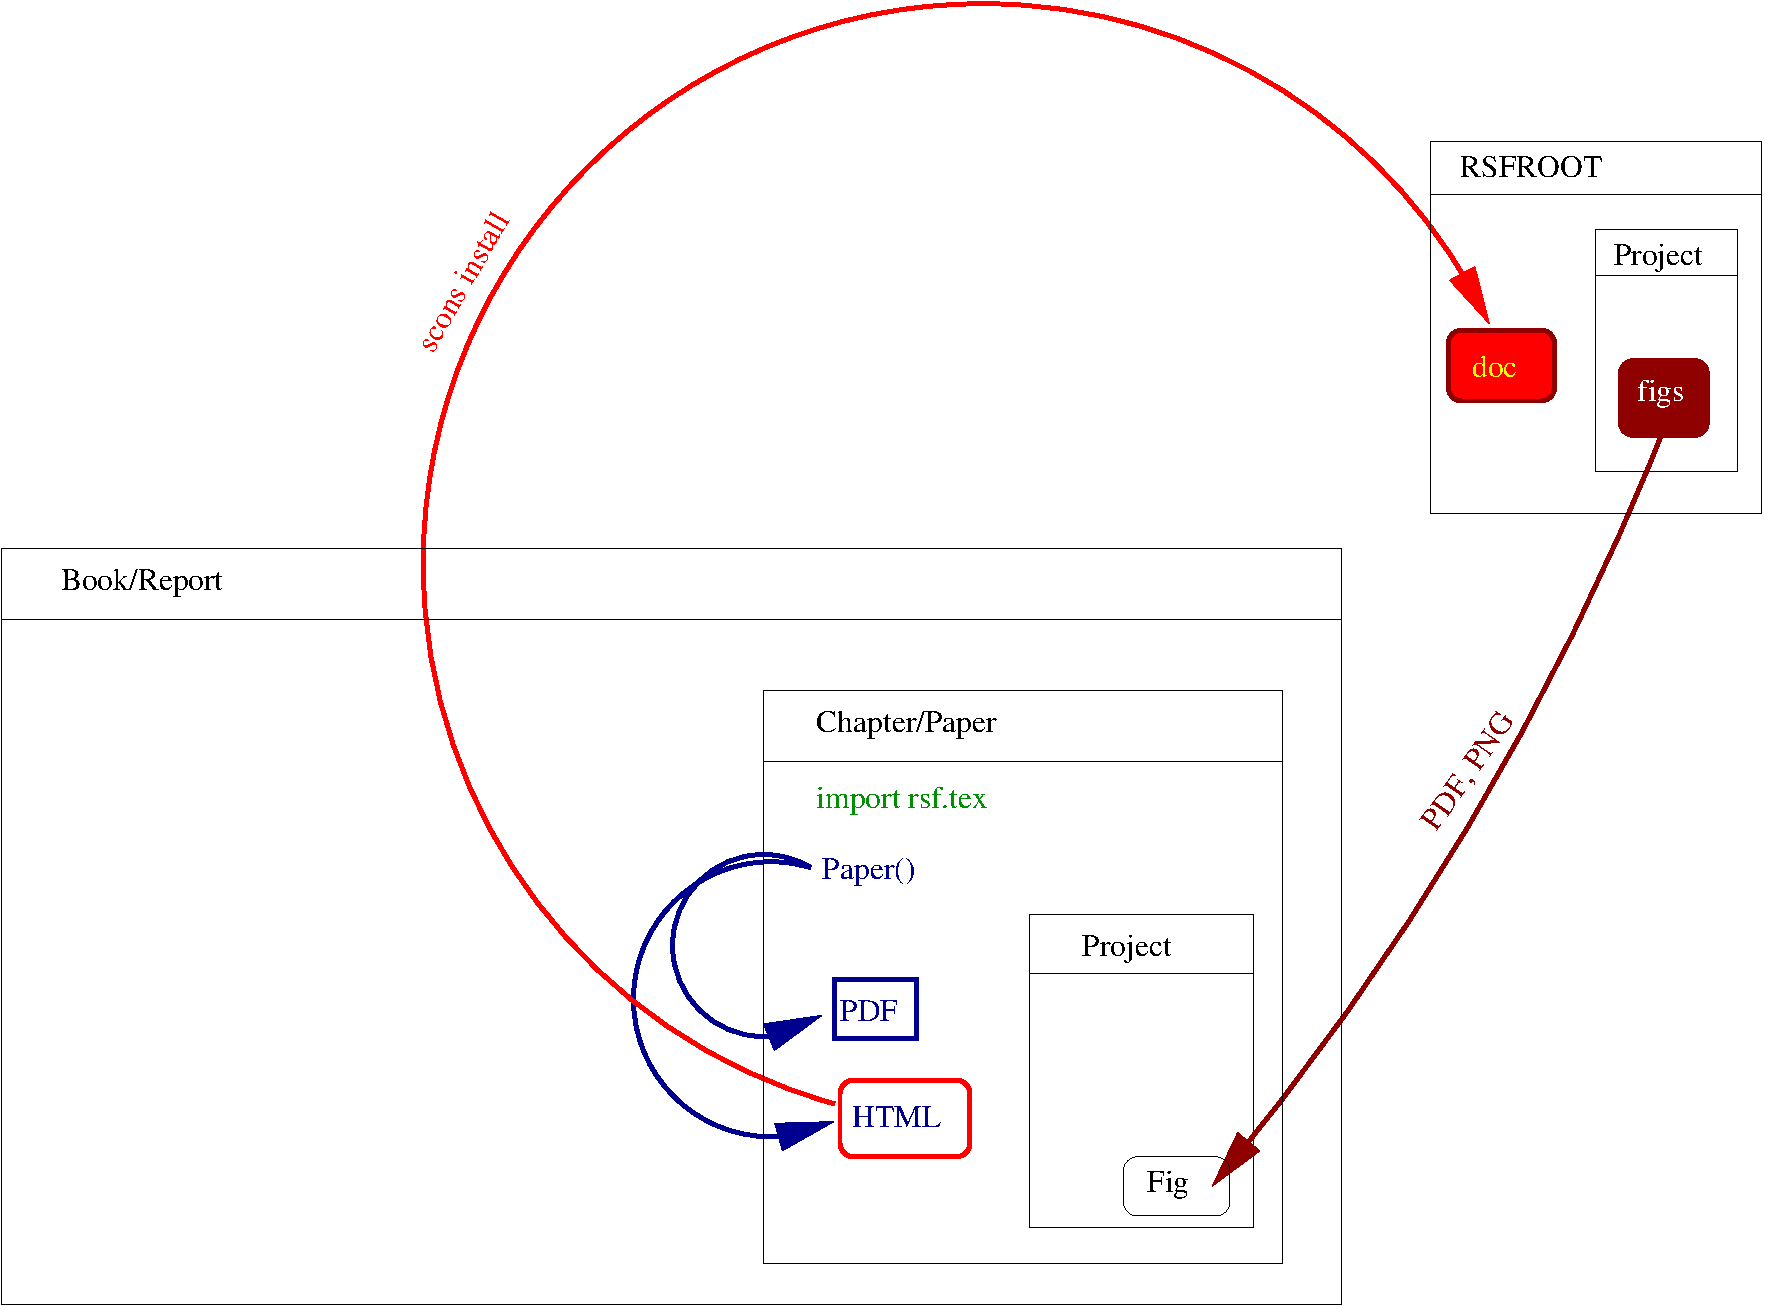
\includegraphics[height=0.8\textheight]{XFig/Fig/scheme2} \\
Courtesy of Fomel (2006)
\end{frame}

\begin{frame}
  \frametitle{{\LaTeX}}
\big{
 \begin{itemize}
    \item Documentation system  
    \item Extends \TeX
    \begin{itemize}
    \item ``Open source''
    \item ``Reproducible''
   \end{itemize}
\item Descriptive language
    \end{itemize}
}
\end{frame}

% ------------------------------------------------------------
\begin{frame} 

\frametitle{The essential tool}

\big{
LeTeX and specifically SEGTeX macros including SEG.bib \\
\begin{itemize}
\item article class.
\item Geophysics class.
\item segabs.cls for SEG abstracts.
\end{itemize}
}
downloading: svn co \url{https://segtex.svn.sourceforge.net/svnroot/segtex/trunk texmf}

\end{frame}
\cwpnote{}


\begin{frame}
  \frametitle{SEGTeX}
  \begin{itemize}
  \item {\LaTeX2e} package
  \item In development 2001--Present
  \item {\color{blue}{\url{http://reproducibility.org/wiki/Main_Page}}}
  \item Multiple purpose
    \begin{itemize}
    \item \emph{Geophysics} papers
    \begin{itemize}
    \item Manuscript style
    \item Publication style 
    \end{itemize}
    \item SEG expanded abstracts
    \item Other
    \begin{itemize}
    \item books and reports
    \item EAGE publications
    \item presentations
     \end{itemize}
    \end{itemize}
   \end{itemize}
\end{frame}

\begin{frame}
  \frametitle{Look Inside SEGTeX}
  \begin{itemize}
  \item \texttt{texmf/}
    \begin{itemize}
    \item \texttt{ls-R} (update with \texttt{texconfig rehash}) 
    \item \texttt{tex/latex/seg/}

    \begin{itemize}
    \item \texttt{geophysics.dtx} (literate programming)
    \item \texttt{geophysics.cls}
    \item \texttt{seg.sty}
    \item $\cdots$
    \end{itemize}

    \item \texttt{bibtex/bst/seg/}

     \begin{itemize}
    \item \texttt{seg.bst}
    \item \texttt{seglike.bst} (Joerg Schleicher)
    \end{itemize}

    \item \texttt{bibtex/bib/seg/}

    \begin{itemize}
    \item \texttt{SEG2005.bib}
    \item \texttt{SEG.bib}
    \end{itemize}

    \item {\texttt{latex2html/}}
    
    \begin{itemize}
    \item \texttt{perl/geophysics.perl}
    \item \texttt{icons/}
    \item \texttt{style.css}
    \end{itemize}

    \end{itemize}    
  \end{itemize}
\end{frame}


% ------------------------------------------------------------
%\begin{frame} 
%
%\frametitle{Installation}
%
%\big{
%\begin{itemize}
%\item Put the contents of the texmf folder where LaTeX can find it
%  (i.e. \$HOME/texmf or specifically \$HOME/texmf/tex/latex)
%\item Run texhash or texconfig.
%\end{itemize}
%}
%
%\end{frame}
%\cwpnote{}

% ------------------------------------------------------------
\begin{frame} 

\frametitle{Where are the live papers?}

\big{In the Madagascar file system: \\
RSFSRC/book \\
$\overbrace{\text{book}}^{main}/\overbrace{\text{sep}}^{group}/\overbrace{\text{banana}}^{paper}/\overbrace{\text{kernel}}^{examples}/\overbrace{\text{Fig}}^{Figures}$
}

\end{frame}
\cwpnote{}

% ------------------------------------------------------------
\begin{frame} 

\frametitle{Paper directory}

\big{
\begin{itemize}
\item paper.tex, paper.bib, SConstruct
\item Fig directory: static plots
\item XFig directory: plots drawn using xfig
\item Math directory: examples using mathematica or matlab
\item marm directory: example using the Marmousi model
\end{itemize}
}

\end{frame}
\cwpnote{}



% ------------------------------------------------------------
\begin{frame} 

\frametitle{Paper: the example subject}

\big{The sensitivity of traveltimes to velocity changes based on (high frequency) rays and (finite frequency) fat rays.}

\end{frame}
\cwpnote{}


\inputdir{kernel}
% ------------------------------------------------------------
\begin{frame} \frametitle{For a ray: the high frequency limit}

\plot{RayKernel}{width=0.9\textwidth}{}
Courtesy of Rickett (2000)
 \end{frame}
\cwpnote{}

% ------------------------------------------------------------
\begin{frame} \frametitle{At 30 Hz}

\plot{BananaPancake8}{width=0.9\textwidth}{}
Courtesy of Rickett (2000)
 \end{frame}
\cwpnote{}

% ------------------------------------------------------------
\begin{frame} \frametitle{At 120 Hz}

\plot{BananaPancake2}{width=0.9\textwidth}{}
Courtesy of Rickett (2000)
 \end{frame}
\cwpnote{}

% ------------------------------------------------------------
\begin{frame} \frametitle{Paper: scope}

\big{
\begin{itemize}
   \item Finite frequency traveltimes
   \item Modify paper and develop equations
   \item A simple example
   \item Application to the Marmousi example
\end{itemize}
}

\end{frame}
\cwpnote{}


% ------------------------------------------------------------
\begin{frame} \frametitle{The paper template: a Madagascar feature}

\begin{itemize}
   \item From the book directory, or one of your own papers
   \item Read the paper and see if you could form a good introduction
     from that paper.
   \item Copy it to your directory compile it (the whole directory)
   \item Remove unwanted examples and corresponding directories (compile again).
   \item Write your abstract (a road map).
\end{itemize}

\end{frame}
\cwpnote{}

% ------------------------------------------------------------
\begin{frame} \frametitle{For the sensitivity kernels} 

\big{
``Traveltime sensitivity kernels: Banana-doughnuts or just
plain bananas?''
}
\big{James Rickett}

\big{RSFSRC/book/sep/banana}

\end{frame}
\cwpnote{}

% ------------------------------------------------------------
\begin{frame} \frametitle{Perturbation theory}

\big{
\begin{equation}
{\bf \delta T} = {\bf A \; \delta S} \nonumber
\end{equation}
${\bf \delta T}$ traveltime perturbations \\
${\bf \delta S}$ slowness perturbations \\
${\bf A}$ modeling operator
\begin{equation}\label{eqn:tomoray}
\delta T=\int_{\rm ray} \delta s({\bf x}) \;dl \nonumber
\end{equation}
}
		
\end{frame}
\cwpnote{}

% ------------------------------------------------------------
\begin{frame} \frametitle{Born-based traveltime}

\big{
\begin{equation} \label{eqn:timeshift}
\delta T = 
\frac{\int_{t_1}^{t_2} {\dot U}(t) \; \delta U(t) \; dt}
{\int_{t_1}^{t_2} {\ddot U}(t) \; U(t) \; dt} \nonumber
\end{equation}
}
courtesy of Marquering et al. (1999)
\begin{equation}\label{eqn:born}
\delta U_{\rm Born}({\bf x},\omega)=\frac{\omega^2}{4 \pi}
\int_V G_0({\bf x},\omega; {\bf x}')\,U_0({\bf x},\omega; {\bf x}')
\delta s({\bf x}') dV({\bf x}') \nonumber
\end{equation}
		
\end{frame}
\cwpnote{}

% ------------------------------------------------------------
\begin{frame} \frametitle{Rytov traveltime}

\big{
\begin{eqnarray}
{\bf \delta T} = \sum_\omega \frac{F(\omega)}{\omega} \;
\Im \left({\bf \delta \Psi}\right) \nonumber \\
= \sum_\omega \frac{F(\omega)}{\omega} 
\;\Im \left( {\bf R \; \delta S}\right) \nonumber
\end{eqnarray}
\begin{equation} 
\delta \psi_{\rm Rytov} ({\bf x},\omega)  = 
\frac{\delta U_{\rm Born}({\bf x},\omega)}{U_0({\bf x},\omega)} \nonumber
\end{equation}
}
		
\end{frame}
\cwpnote{}

% ------------------------------------------------------------
\begin{frame} 

\frametitle{Getting started}
\vspace{-.6in}
\big{\begin{itemize}
\item Copy the directory ``book/sep/banana'' to your desired location
\item cp -r book/sep/banana ~/.
\item Change directory name (i.e. doughnut)
\item enter the directory
\item Compile the paper: ``sftour scons lock'' and then ``scons read''
\end{itemize}
}

\end{frame}
\cwpnote{}

% ------------------------------------------------------------
\begin{frame} 

\frametitle{Compiling options}

\big{\begin{itemize}
\item scons paper.read
\item scons paper.pdf
\item scons paper.html
\item scons paper.wiki
\end{itemize}
}

\end{frame}
\cwpnote{}

% ------------------------------------------------------------
\begin{frame} \frametitle{The paper SConstruct}

\big{SConstruct}
\normalsize 
\lstinputlisting[firstline=1,lastline=12]
		{SConstruct}
		
\end{frame}
\cwpnote{}

% ------------------------------------------------------------
\begin{frame} 

\frametitle{Make a change: reproducible?}

\big{\begin{itemize}
\item Look at the paper
\item Access its tex version
\item and especially the Figures
\end{itemize}
}

\end{frame}
\cwpnote{}

% ------------------------------------------------------------
\begin{frame} \frametitle{paper.tex}

\normalsize 
\lstinputlisting[firstline=1,lastline=15]
		{paper.tex}
		
\end{frame}
\cwpnote{}

% ------------------------------------------------------------
\begin{frame} \frametitle{paper.tex}

\big{The Figures directory}
\normalsize 
\lstinputlisting[firstline=189,lastline=194]
		{paper.tex}
		
\end{frame}
\cwpnote{}

% ------------------------------------------------------------
\begin{frame} \frametitle{paper.tex}

\big{Calling the Figure}
\normalsize 
\lstinputlisting[firstline=203,lastline=210]
		{paper.tex}
		
\end{frame}
\cwpnote{}

% ------------------------------------------------------------
\begin{frame} 

\frametitle{Make a change: reproducible?}

\big{\begin{itemize}
\item Enter directory ``kernel''
\item Open SConstruct using your favorite editor
\end{itemize}
}

\end{frame}
\cwpnote{}

% ------------------------------------------------------------
\begin{frame} \frametitle{The example SConstruct}

\big{kernel/SConstruct}
\normalsize 
\lstinputlisting[firstline=1,lastline=12]
		{kernel/SConstruct}
		
\end{frame}
\cwpnote{}

% ------------------------------------------------------------
\begin{frame} \frametitle{Use Born instead of Rytov}

\big{kernel/SConstruct}
\normalsize 
\lstinputlisting[firstline=25,lastline=32]
		{kernel/SConstruct}

\big{code name: sfsensitivity}
		
\end{frame}
\cwpnote{}

% ------------------------------------------------------------
\begin{frame} \frametitle{Modifications}

\big{
\begin{itemize}
   \item Change 6 to 2 using your favorite editor
   \item scons view
   \item scons lock
   \item cd ..; scons read
\end{itemize}
}

\end{frame}
\cwpnote{}

% ------------------------------------------------------------
\begin{frame} \frametitle{Adopting the paper}
\vspace{-.6in}
\big{
\begin{itemize}
   \item Insert new title
   \item Modify author(s)
   \item Change introduction to your language, use references and add this paper as
     a reference ``banana.bib''
   \item Clean the rest, keep one Figure
   \item start writing your own paper
  \item remove examples if not needed
\end{itemize}
}

\end{frame}
\cwpnote{}

% ------------------------------------------------------------
\begin{frame} \frametitle{Adding synthetic examples}
\vspace{-.6in}
\big{
\begin{itemize}
   \item Directory ``RSFSRC/book/data'' or any other paper running an
     example
   \item Copy the example to your paper directory (i.e. \$RSFSRC/book/swag/eikds/smvel)
   \item cd smvel; scons view; scons lock
   \item This forms a start, clean it up and add your code example
\end{itemize}
}

\end{frame}
\cwpnote{}

% ------------------------------------------------------------
\begin{frame} \frametitle{Including the new example}
\vspace{-.6in}
\big{
\begin{itemize}
   \item cd ..
   \item Open paper.tex with you favorite editor
   \item Above the plot call type: \\inputdir\{smvel\}
   \item Insert the Figure name inside the Plot function
   \item modify the caption
   \item reference the Figure in a sentence
   \item Save and compile; scons read
\end{itemize}
}

\end{frame}
\cwpnote{}

% ------------------------------------------------------------
\begin{frame} \frametitle{More info}

\big{
\begin{itemize}
   \item \url{http://www.reproducibility.org/wiki/SEGTeX\#Documentation}
   \item \$RSFSRC/book/rsf
\end{itemize}
}

\end{frame}
\cwpnote{}

% ------------------------------------------------------------
\begin{frame} \frametitle{Tips and tricks }

\big{
\begin{itemize}
   \item Be patient, do not give up
   \item Use rsf-user@lists.sourceforge.net
   \item SConstruct controls everything, try, at least, to understand
   \item Always access other papers with the power of ``grep''
\end{itemize}
}

\end{frame}
\cwpnote{}


% ------------------------------------------------------------
\begin{frame} \frametitle{Reproducible papers }

\url{http://www.reproducibility.org/wiki/Reproducible_Documents}
\url{http://www.reproducibility.org/RSF/book/sep/banana/paper_html/}

\begin{itemize}
   \item Source: \$RSFSRC/book/sep/banana
\end{itemize}

\end{frame}
\cwpnote{}

\inputdir{.}

% ------------------------------------------------------------
\begin{frame} \frametitle{Documentation}

\big{
Madagascar Programming Reference Manual}
\big{courtesy of SWAG}
\big{RSFSRC/book/rsf/manual}

\end{frame}
\cwpnote{}

% ------------------------------------------------------------
\begin{frame} \frametitle{Content}

\begin{itemize}
   \item Covers all available data types and subroutines under rsf.h
   \item Includes a description (beyond what was given by the developer)
   \item It organizes them in terms of usage and purpose
   \item we plan to have the manual get built automatically to include
     updates in the subroutine
 \item \$RSFSRC/book/rsf/manual
\end{itemize}

\end{frame}
\cwpnote{}

% ------------------------------------------------------------
\begin{frame} \frametitle{Content}\
\vspace{-0.2in}

\begin{itemize}
\item \emph{An example: Finite-Difference modeling}
\item \emph{Data types}\label{sec:datatypes}
\item \emph{Preparing for input}\label{sec:input}
\item \emph{Operations with RSF files}\label{sec:files}
\item \emph{Error handling}\label{sec:error}
\item \emph{Linear operators}\label{sec:lop}
\item \emph{Data analysis}\label{sec:analysis}
\item \emph{Filtering}\label{sec:filter}
\item \emph{Solvers}\label{sec:solvers}
\item \emph{Interpolation}\label{sec:interpolation}
\item \emph{Smoothing}\label{sec:smoothing}
\item \emph{Ray tracing}\label{sec:ray}
\item \emph{General tools}\label{sec:general}
\item \emph{Geometry}\label{sec:geometry}
\item \emph{Miscellaneous}\label{sec:misc}
\item \emph{System}\label{sec:system}
\end{itemize}
\end{frame}
\cwpnote{}


% ------------------------------------------------------------
\begin{frame} \frametitle{Pointers}

\big{
\begin{itemize}
   \item Be patient, do not give up
   \item Use rsf-user@lists.sourceforge.net
   \item SConstruct controls everything, try, at least, to understand it
   \item You could always run RSF like SU
\end{itemize}
}

\end{frame}
\cwpnote{}

% ------------------------------------------------------------
\begin{frame} \frametitle{Final remarks}

\big{
\begin{itemize}
   \item Make things simple
   \item Get to know Madagascar, it can be your friend, but hopefully
     not your only friend
   \item Always compile (makes error search easier)
   \item Reproducible is good (very good)
   \item Love thy neighbor $\rightarrow$ contribute
\end{itemize}
}

\end{frame}
\cwpnote{}


% ------------------------------------------------------------
\begin{frame}

\big{I thank the supporters of SWAG}

\vfill

\begin{center}
\plot{swag_logo}{width=0.3\textwidth}{}
%\pgfuseimage{../Fig/swag_logo}
\end{center}

\big{\url{http://swag.kaust.edu.sa}}

\end{frame}

\cwpnote{}


%% 
 % contest: nicest impulse response at z=7km, x=14km
 % beauty: 1...100 (nicest image, i.e. fewest artifacts)
 % cost:   1...100 (highest cost, i.e. most receivers)
 % find the highest b/c score
 %%
